\documentclass[11pt]{article}

\usepackage[utf8]{inputenc}
\usepackage{pgfplots}
\pgfplotsset{compat=1.18, width=10cm}

\begin{document}

\section{2D Plots}

% https://www.youtube.com/watch?v=5jmIHOWpEg0&ab_channel=Dr.TreforBazett
% Dr. Trefor Bazett - How I make beautiful GRAPHS and PLOTS using LaTeX
% full docs: https://www.iro.umontreal.ca/~simardr/pgfplots.pdf

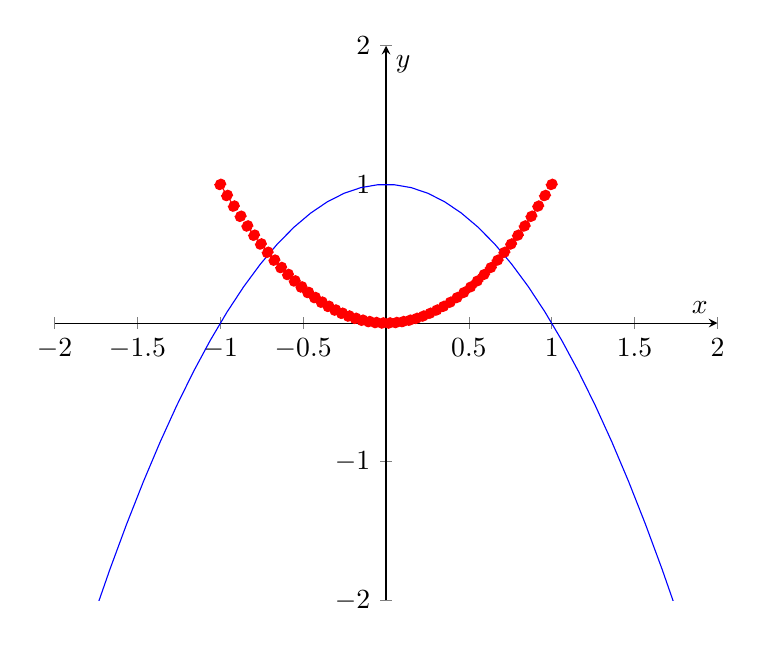
\begin{tikzpicture}
\begin{axis}[xmin=-2, xmax=2, ymin=-2, ymax=2, axis lines=middle, xlabel=$x$, ylabel=$y$]
\addplot[color=red, dashed, mark=*, samples=50, domain=-1:1]{x^2};
\addplot[color=blue, samples=100]{1-x^2};
\end{axis}
\end{tikzpicture}\\[10pt]

\begin{tikzpicture}
    \begin{axis}[clip=false,
        xmin=0, xmax=2.5*pi,
        ymin=-1.5, ymax=1.5,
        axis lines=middle,
        xtick={0, pi/2, pi, 3*pi/2, 2*pi},
        xticklabels={$0$, $\frac{\pi}{2}$, $\pi$, $\frac{3\pi}{2}$, $2\pi$},
        xticklabel style={anchor=south west},
        xmajorgrids=true,
        grid style=dashed,
        ]
        \addplot[domain=0:2*pi,red]{sin(deg(x))}node[right,pos=0.9]{$f(x)=\sin x$};
        \addplot[domain=0:2*pi,,blue]{cos(deg(x))}node[right,pos=1]{$g(x)=\cos x$};
    \end{axis}
\end{tikzpicture}\\[10pt]

\begin{tikzpicture}
\begin{axis}
\addplot+[
    only marks,
    scatter,
    mark size=2.9pt]
table[meta=ma]
{test.txt};
\end{axis}
\end{tikzpicture}\\[10pt]

% \begin{tikzpicture}
% \begin{axis}
% \addplot+[
%     only marks,
%     scatter,
%     mark size=2.9pt
% ] coordinates {
%     (5,8.312e-02) (17,2.547e-02) (49,7.407e-03)
%     (129,2.102e-03) (321,5.874e-04) (769,1.623e-04)
%     (1793,4.442e-05) (4097,1.207e-05) (9217,3.261e-06)
% };
% \end{axis}
% \end{tikzpicture}\\[10pt]

% \begin{tikzpicture}
% \begin{axis}
% \addplot+[
%     only marks,
%     scatter,
%     mark size=2.9pt
% ]
% {rand};
% \end{axis}
% \end{tikzpicture}\\[10pt]

\begin{tikzpicture}
\begin{axis}[scatter/classes={
a={mark=square*,blue},%
b={mark=triangle*,red},%
c={mark=o,draw=black}}]
% \addplot[] is better than \addplot+[] here:
% it avoids scalings of the cycle list
\addplot[scatter,only marks,
scatter src=explicit symbolic]
coordinates {
(0.1,0.15) [a]
(0.45,0.27) [c]
(0.02,0.17) [a]
(0.06,0.1) [a]
(0.9,0.5) [b]
(0.5,0.3) [c]
(0.85,0.52) [b]
(0.12,0.05) [a]
(0.73,0.45) [b]
(0.53,0.25) [c]
(0.76,0.5) [b]
(0.55,0.32) [c]
};
\end{axis}
\end{tikzpicture}

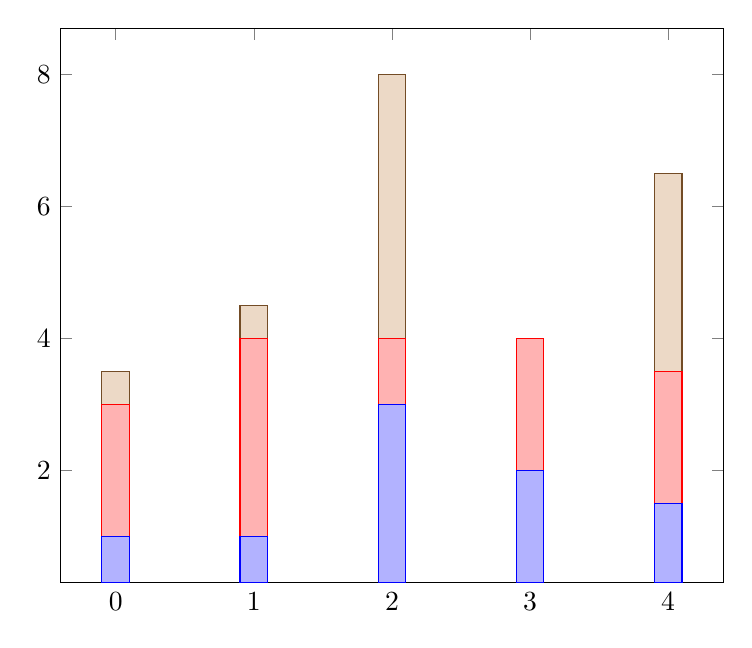
\begin{tikzpicture}
\begin{axis}[ybar stacked]
\addplot coordinates
{(0,1) (1,1) (2,3) (3,2) (4,1.5)};
\addplot coordinates
{(0,2) (1,3) (2,1) (3,2) (4,2)};
\addplot coordinates
{(0,0.5) (1,0.5) (2,4) (3,0) (4,3)};
\end{axis}
\end{tikzpicture}

\section{3D Plots}

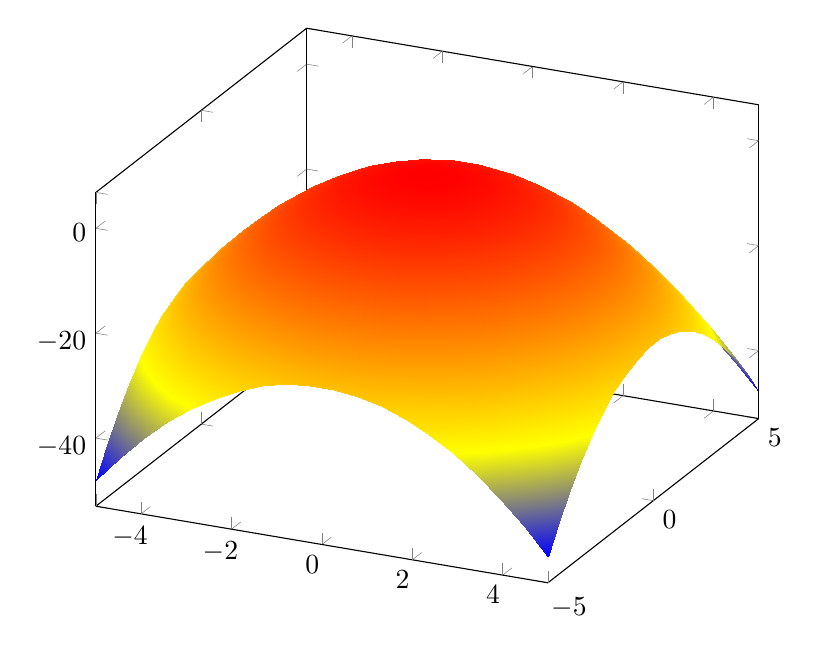
\begin{tikzpicture}
\begin{axis}
\addplot3[surf, samples=20, shader=interp]{2-x^2-y^2};
\end{axis}
\end{tikzpicture}\\[10pt]

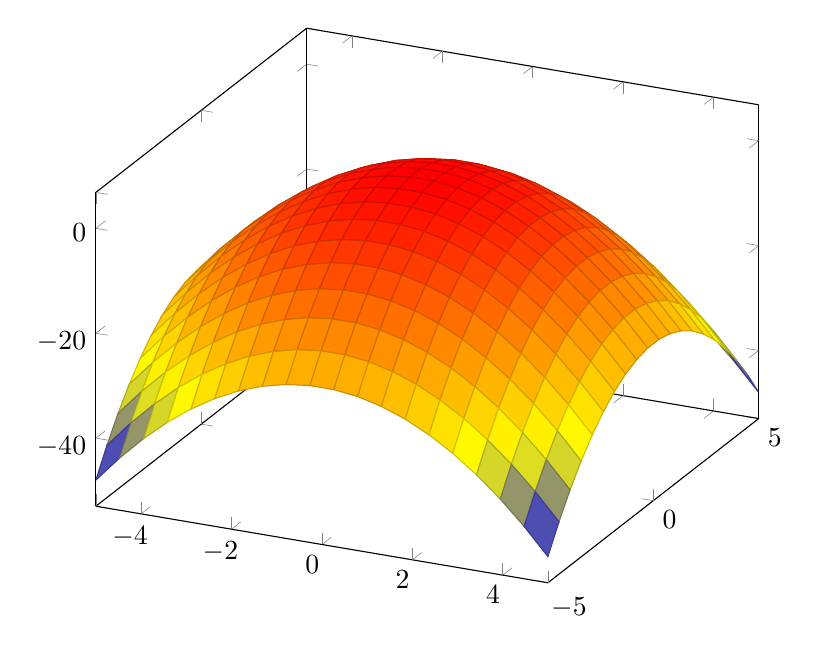
\begin{tikzpicture}
\begin{axis}
\addplot3[surf, samples=20]{2-x^2-y^2};
\end{axis}
\end{tikzpicture}\\[10pt]

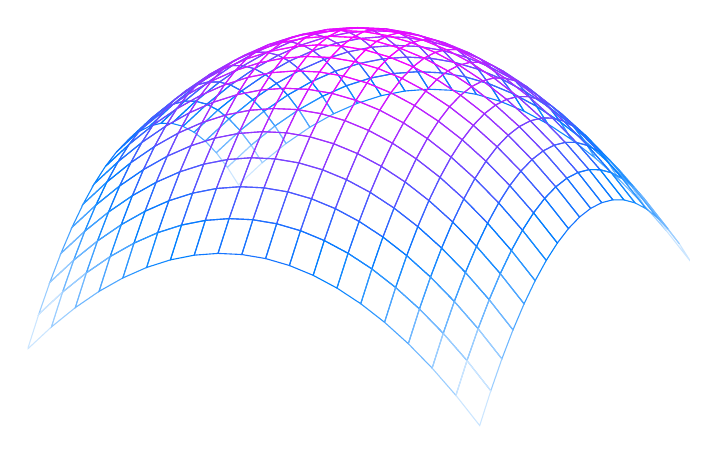
\begin{tikzpicture}
\begin{axis}[colormap/cool, hide axis]
\addplot3[mesh, samples=20]{2-x^2-y^2};
\end{axis}
\end{tikzpicture}\\[10pt]

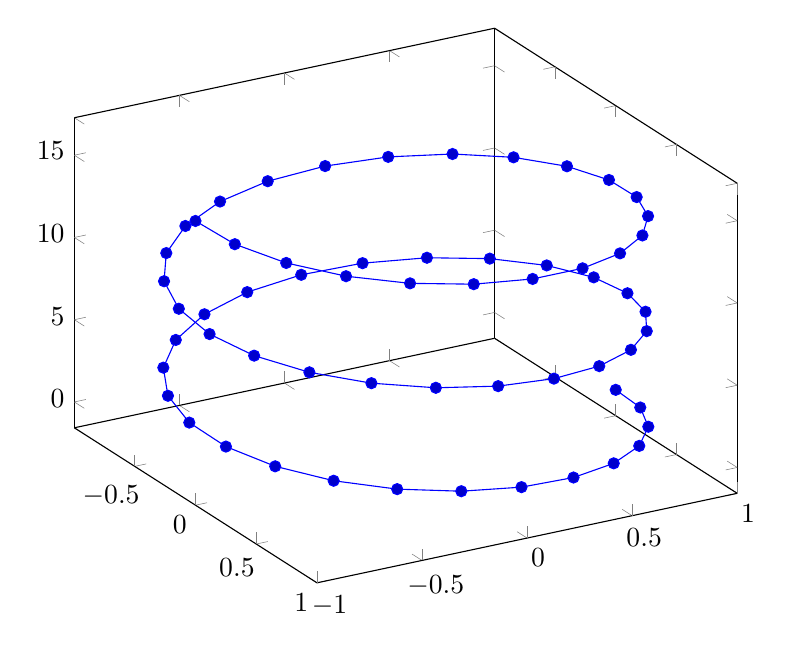
\begin{tikzpicture}
\begin{axis}[view={60}{30}]
\addplot3+[domain=0:5*pi,samples=60,samples y=0]
({sin(deg(x))},
{cos(deg(x))},
{x});
\end{axis}
\end{tikzpicture}\\[10pt]

\end{document}